\chapter{Robots Móviles y Agentes Inteligentes}


\section{Máquina de Estado}

\begin{itemize}
	\item[\textbullet] Entradas
	\item[\textbullet] Máquinas
	\item[\textbullet] Salidas
\end{itemize}

\section{Máquina de Estado Aumentada}

Una entrada (o salida) de una máquina puede ser sustituida por la salida de otra máquina de estados. Esa bloquea la entrada (o salida) ordinaria y pone su salida.

\begin{figure}[h!]
	\centering
	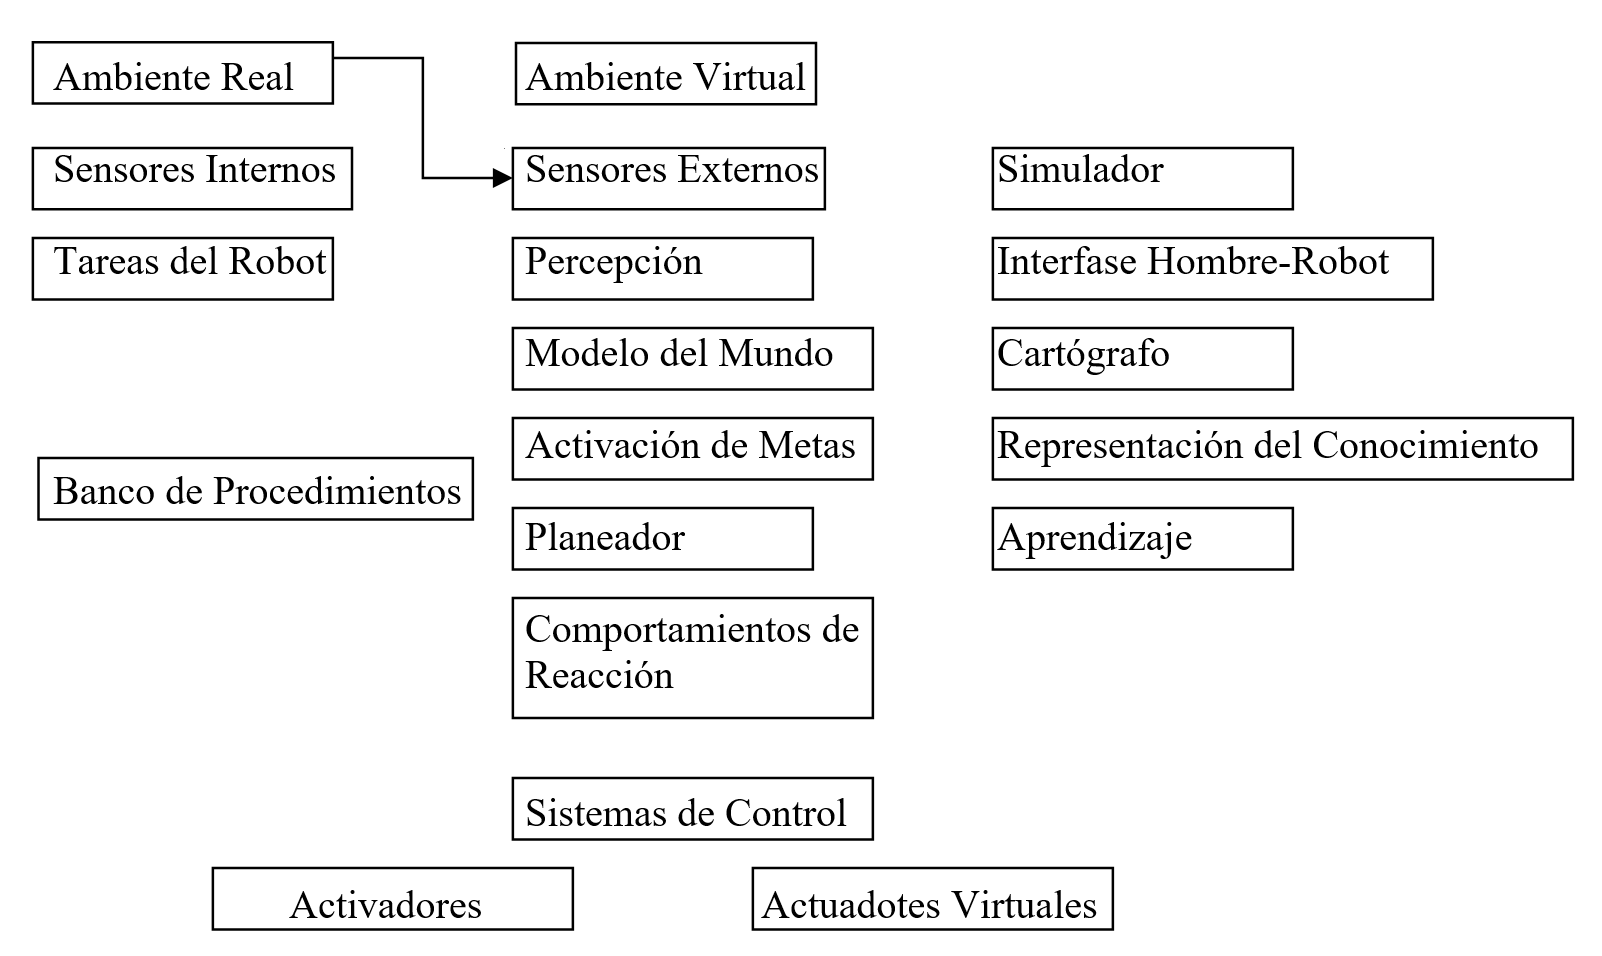
\includegraphics[width=0.5\textwidth]{images/img49.png}
	\label{figura49}
\end{figure}

\section{Arquitecturas Reactivas (o por Comportamientos)}

Diagramas de Stimulus Response (SR)

\begin{figure}[h!]
	\centering
	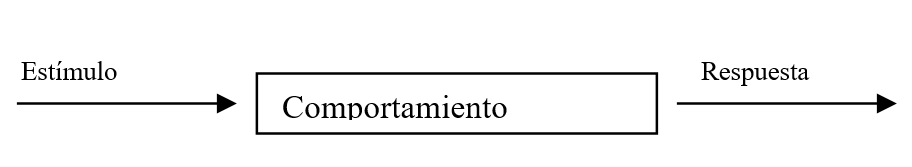
\includegraphics[width=0.5\textwidth]{images/img50.png}
	\label{figura50}
\end{figure}

La idea es que la respuesta sea instantánea.
En los comportamientos puros, la respuesta únicamente depende del estímulo.

\subsection{Organización de los comportamientos:} 

\textit{Esquema 1}

\begin{figure}[h!]
	\centering
	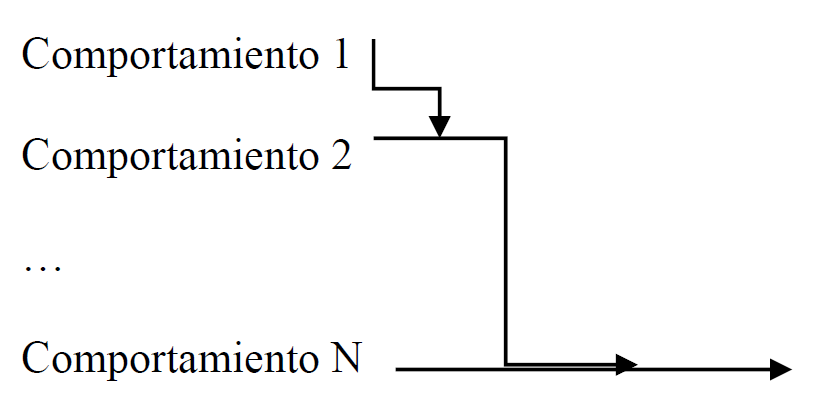
\includegraphics[width=0.5\textwidth]{images/img51.png}
	\label{figura51}
\end{figure}


Algunos comportamientos bloquean la salida de otros. Solamente la salida de uno es el que se usa, todos se activan. El diagrama anterior decide la prioridad.

La salida generalmente es un vector que, por ejemplo, indica la magnitud y dirección del movimiento del robot.

\textit{Esquema 2}

\begin{figure}[h!]
	\centering
	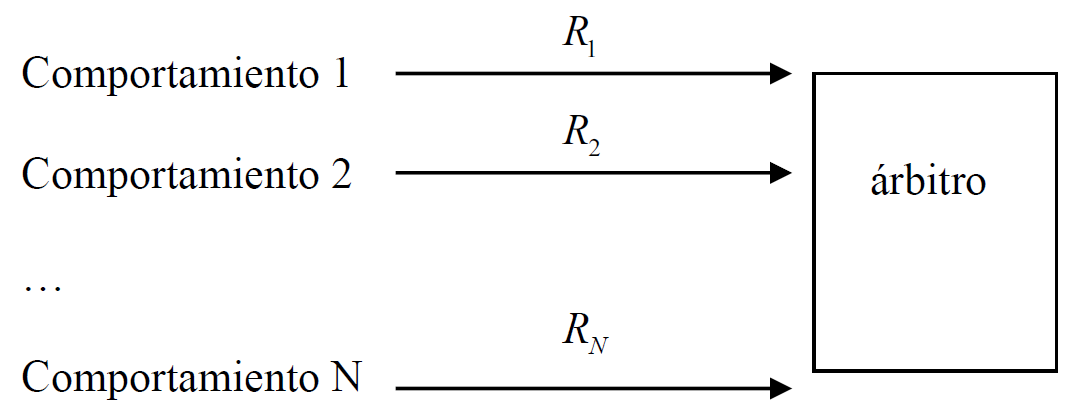
\includegraphics[width=0.5\textwidth]{images/img52.png}
	\label{figura52}
\end{figure}


El árbitro decide cuál es la respuesta.

\begin{figure}[h!]
	\centering
	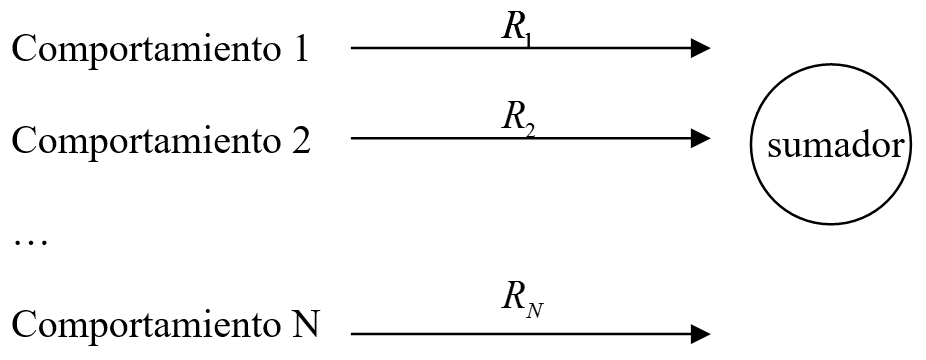
\includegraphics[width=0.5\textwidth]{images/img53.png}
	\label{figura53}
\end{figure}


El sumador hace un promedio ponderado por\textit{ganancias}.

$$
\sum_{i=1}^{N} \, g_i \, R_i
$$

La ganancia depende del diseñador y va a hacer que el robot se comporte de diferente forma (robot “audaz” contra robot “conservador”).

Un diagrama del espacio se puede hacer con campos vectoriales (diagramas de flechitas tipo sistemas dinámicos), por ejemplo uno que sea de las fuerzas de atracción y otro de repulsión y sumarlos.

Puedo tener una complejidad grande combinando comportamientos, pues pueden controlar diferentes cosas.


\section{Máquinas de Estado}
\subsection{Algoritmo para el Comportamiento de Evadir Obstáculos}

Un robot circula con:

\begin{itemize}
	\item[\textbullet] Dos motores, uno a cada lado.
	\item[\textbullet] Dos sensores adelante, para detectar obstáculos (por ejemplo, infrarrojos, ultrasonido, etc.)
\end{itemize}

\begin{figure}[h!]
	\centering
	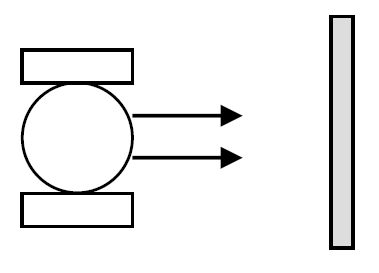
\includegraphics[width=0.5\textwidth]{images/img54.png}
	\label{figura54}
\end{figure}

Obviamente:
\begin{itemize}
	\item[\textbullet] Si los sensores no detectan el obstáculo, seguir 		avanzando.
	\item[\textbullet] Si el sensor derecho lo detecta y el otro no, hacerlo tantito para atrás y girar hacia la izquierda para seguir avanzando
	\item[\textbullet]Si el sensor izquierdo lo detecta y el otro no, hacerlo tantito para atrás y girar hacia la derecha para seguir avanzando
	\item[\textbullet]Si los dos detectan, hacerlo para atrás y giro 90°.
\end{itemize}

\begin{figure}[h!]
	\centering
	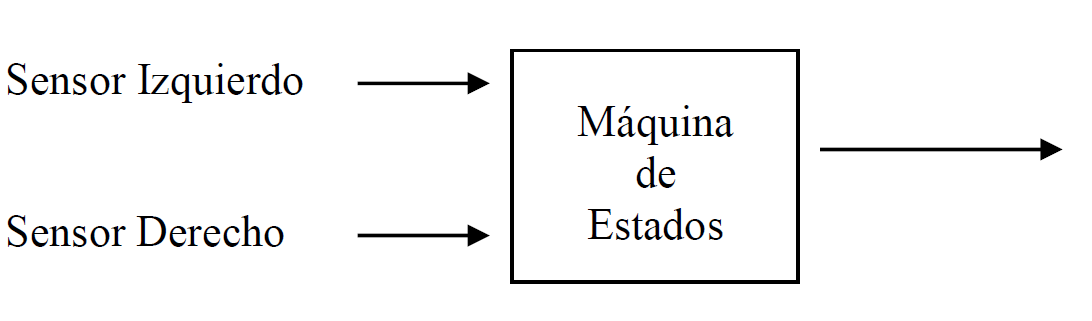
\includegraphics[width=0.5\textwidth]{images/img55.png}
	\label{figura55}
\end{figure}


\textit{Notación de diagrama de flujo}


\begin{figure}[h!]
	\centering
	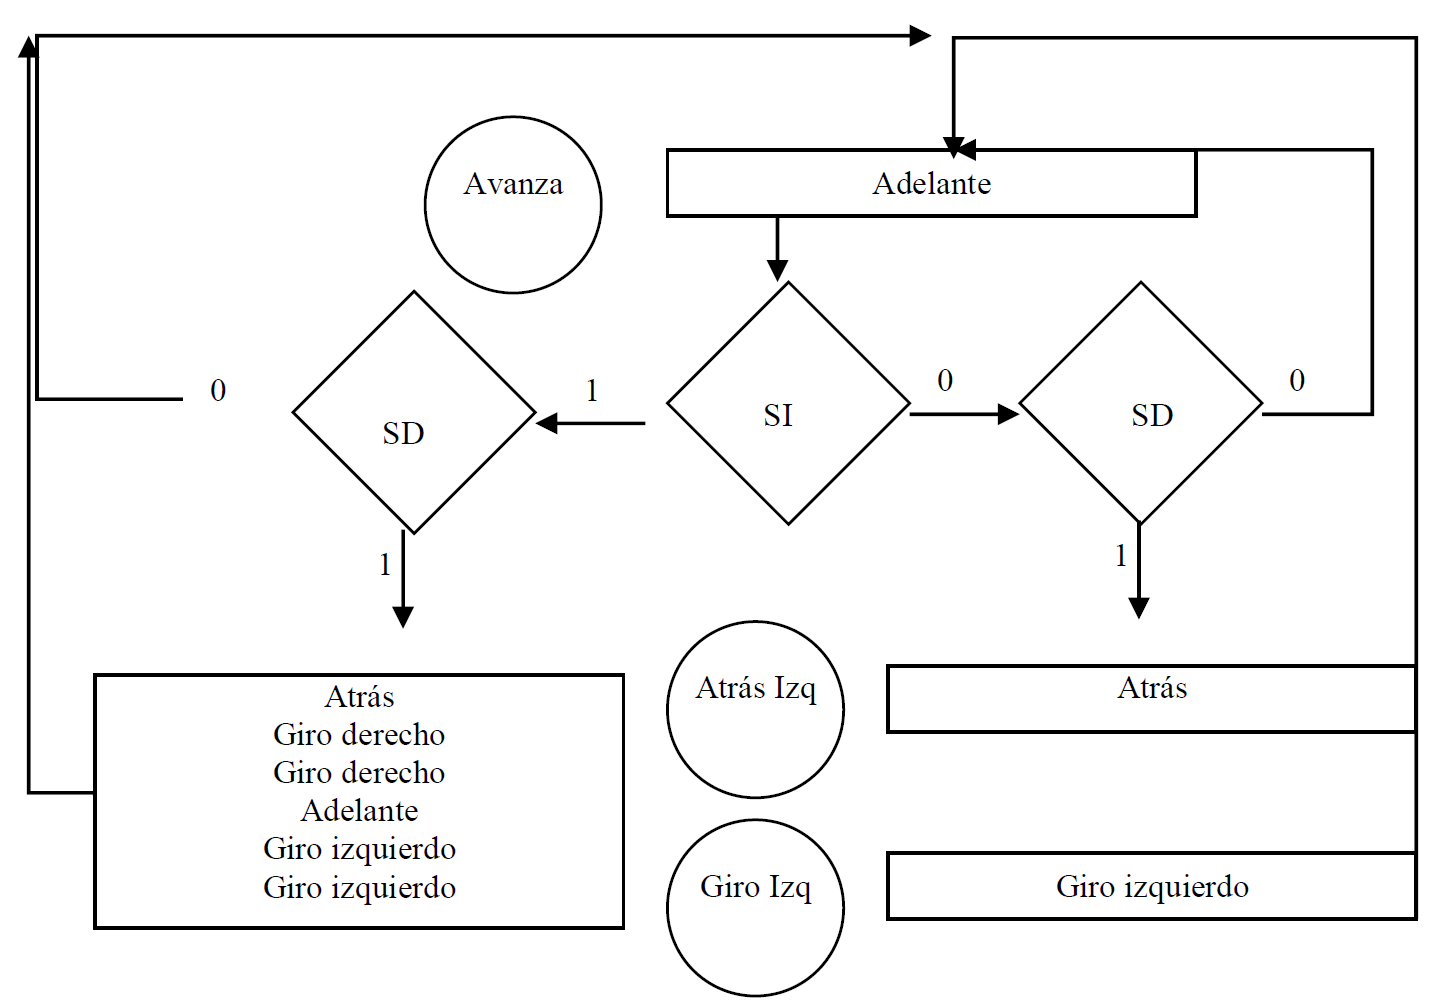
\includegraphics[width=0.5\textwidth]{images/img56.png}
	\label{figura56}
	
\end{figure}
\break

Si se quisiera programar esto con una subrutina, hace todo.  En la teoría de comportamientos necesito una respuesta inmediata y necesito que cuando vuelva a entrar se guarde el estado.

\section{AFSM (Augmented Finite State Machine)}

La máquina de estados aplicada a robots representa el comportamiento.
Una máquina tradicional de estados tiene entradas y salidas.
Rodney Brooks (MIT) inventó la máquina de estados finitos aumentada.

Básicamente el concepto es que alguna de las entradas es inhibida por otra máquina de estados (su salida se convierte la entrada) y en las salidas están los supresores, que bloquean la salida de la máquina y colocan un valor. Por último hay una entrada de “reset” que hace que se coloque en un estado en específico.

Con AFSM podemos tener diferentes capas y hacer una respuesta \textbf{jerárquica}.

\begin{figure}[h!]
	\centering
	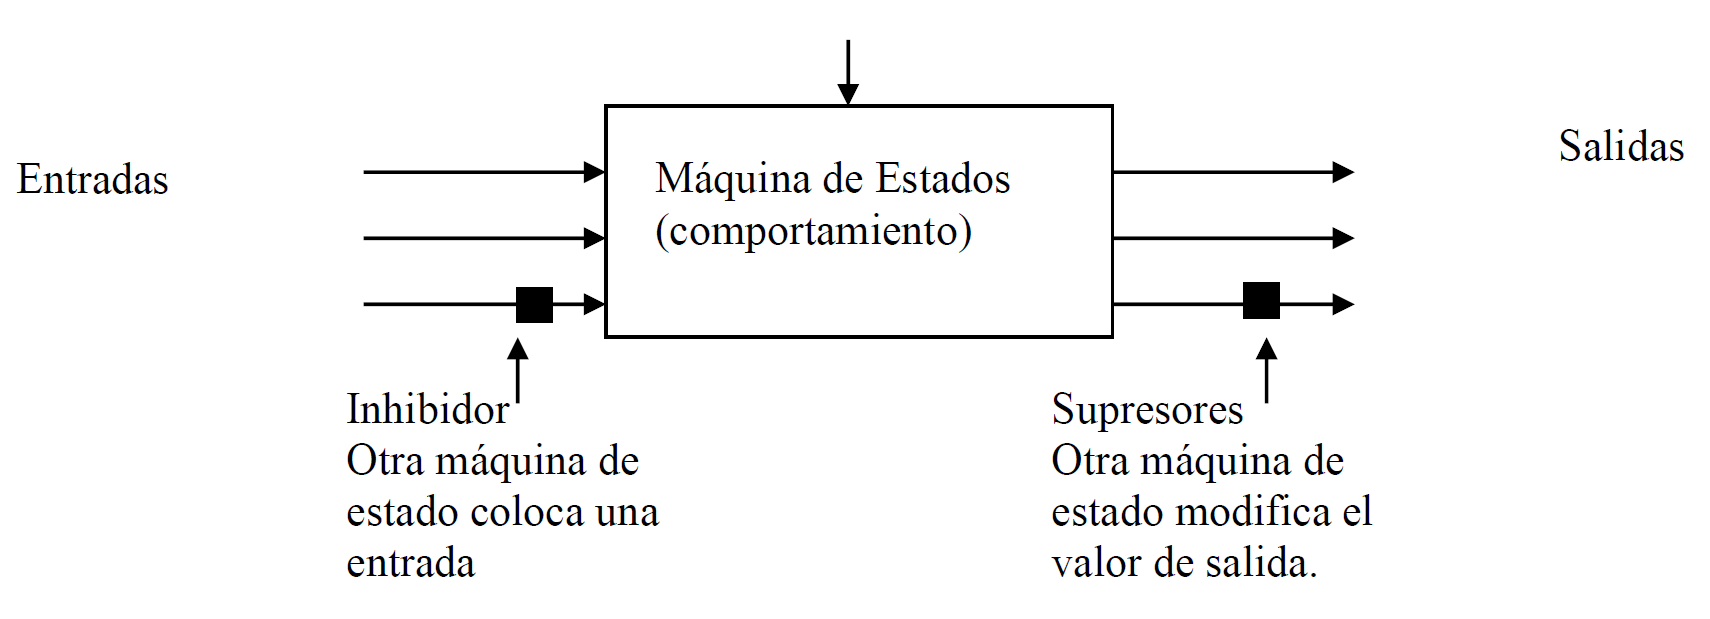
\includegraphics[width=0.5\textwidth]{images/img57.png}
	\label{figura57}
	
\end{figure}
\break

\section{Campos Potenciales}

Se modela el robot como una canica. Los obstáculos ahora son montañas que ejercen fuerzas de repulsión. El destino es un hoyo.
El robot se mueve a través de un campo potencial por la pendiente más pronunciada hasta que lo lleva al destino.

\begin{figure}[h!]
	\centering
	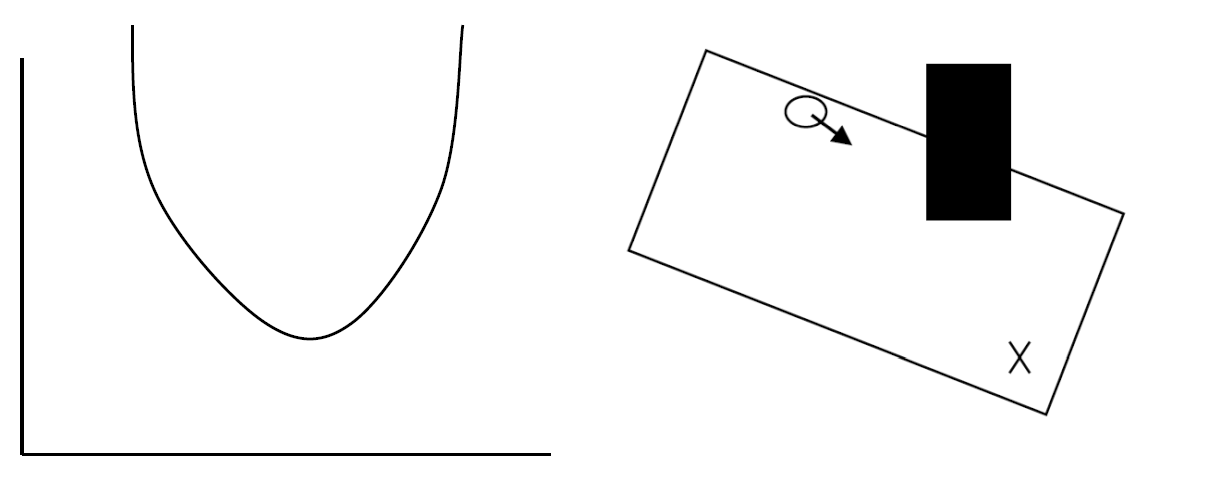
\includegraphics[width=0.5\textwidth]{images/img58.png}
	\label{figura58}
\end{figure}

$$
y=y_0 + (x-x_0)^2
$$


El mínimo se encuentra diferenciando.
$$
\dfrac{\partial y}{\partial x} = 2(x-x_0)
$$
$$
x^* = x_0
$$

Supongamos que no se conoce la ecuación; entonces se utiliza un método iterativo.
Empiezo con un punto $x_{n-1}$ cualquiera y dependiendo del valor de la pendiente me muevo hacia la izquierda o la derecha.

Es una relación de recurrencia:

\begin{center}
	$ x_n= \int(x_{n-1}) = x_{n-1} - \partial \dfrac{\partial y}{\partial x} $ \,  donde $\partial$ es una constante.	
\end{center}

\textbf{Por ejemplo:} \\
Si consideramos $\delta = \dfrac{1}{2}$ se tiene $x_n = x_{n-1} \, \dfrac{-1}{2}(2(x_{n_1}-x_0)) = x_0$.


Esto da pie a considerar la situación general.

\textbf {Se utiliza Steepest Descent.} 

\textit{Posición del robot en n:} $q_n = \left[x_n,y_n\right]^T$
$$
q_n=q_{n-1}-\delta f (q_{n-1}) $$

donde $f(z)= \dfrac{F(z)}{\|F(z)\|} = U(z)$ y $U(z)$  es el campo potencial del medio ambiente en donde navega el robot $U(z)= U_{atr}(z) + U_{rep}(z)$ (dos componentes, uno atractor y un repulsor).

Al final se tienen fuerzas de atracción más fuerzas de repulsión.

Se define:

$U_{atr} = \dfrac{1}{2} \, \varepsilon_1 \,  \|q-q_{dest}\|^2 $(campo de tipo parabólico) donde $q_{dest}$  es la posición del destino. 
Se ve claro que es parabólico:

$$
U_{atr}=\frac{1}{2} \, \varepsilon_1(x-x_{dest})^2 + (y-y_{dest})^2
$$
La fuerza de atracción en q es:

$$
\nabla U_{atr}= \varepsilon_1 \begin{bmatrix}(x-x_{dest}) \\ (y-y_{dest}) \end{bmatrix} = \varepsilon_1[q-q_{dest}] = F_{atr}(q)
$$



La fuerza de atracción se va a convertir en aceleración. Para fuerzas muy grandes se transforma en aceleraciones muy grandes. 
Esto no se quiere, por lo que se tiene un umbral. Esta fórmula solamente aplica para $\|q-q_{dest}\| < d_1$.

¿Qué pasa en $\|q-q_{dest}\|>d_1$?

$$
U_{atr}=E_2\|q-q_{dest}\|
$$

Esto es un campo cónico:

$$
U_{atr}=E_2\sqrt{(x-x_{dest})^2 + (y-y_{dest})^2)}
$$

$$
\nabla U_{atr} = E_2 \begin{bmatrix} \dfrac{(x-x_{dest})}{\sqrt{(x-x_{dest})^2+(y-y_{dest})^2}} \\ 
\dfrac{(y-y_{dest})}{\sqrt{(x-x_{dest})^2+(y-y_{dest})^2}}
\end{bmatrix} = \dfrac{E_2}{\rVert q-q_{dest}\lVert}
\begin{bmatrix}
x-x_{dest} \\
y-y_{dest}
\end{bmatrix} = E_2 \dfrac{q-q_{dest}}{\lVert q-q_{dest}\rVert}
$$

Campos Repulsivos

¿Cómo representar el obstáculo? Se podría considerar un solo vector en el centroide, una serie de puntos que ejercen repulsión, etc. Depende del diseñador.

$$U_{rep}(q)=\frac{1}{2}\eta \left( \dfrac{1}{\lVert q-q_{obs}\rVert} - \dfrac{1}{d_0} \right) ^2 $$

Esto aplica cuando $q-q_{obs}$. En caso contrario, se toma como 0. Esto es para que no lo tomes en cuenta si está demasiado lejos.

$$
\nabla U_{rep}(q)=-\dfrac{\eta}{\rVert q-q_{obs}\lVert ^2} \left( \dfrac{1}{\lVert q-q_{obs}\rVert} - \dfrac{1}{d_0} \right)
\left( \dfrac{q-q_{dest}}{\lVert q-q_{dest}\rVert}\right)
 =F_{rep}(q)
$$

En general,

$$
F(q)=F_{atr}(q)+\sum_{i=1}^{n}\, F_{rep}(q)
$$

$$
f(q)=\frac{F(q)}{\|F(q)\|}=\nabla U(q)
$$

$$
q_{i+1}=q_i - \delta_i f(q_i)
$$

\begin{figure}[h!]
	\centering
	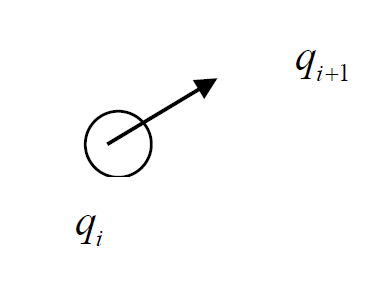
\includegraphics[width=0.3\textwidth]{images/img59.png}
	\label{figura59}
\end{figure}



\begin{ejemplo}
	Robot:(1,1) \\
	Obstáculo: hexágono centrado en (2,2) \\
	Objetivo:(5,4) \\
	$q_0=(1,1)$\\
	Se va a tomar $d_0=	5, \varepsilon_1=1, \eta=2,\delta_0=1$ y se va a utilizar la parabólica
\end{ejemplo}

Se tiene: 
$$
F_{atr}(q_0) = \varepsilon_1 (q_0-q_{dest}) = (-4,-3)
$$

$$
F(q_0) = - \dfrac{\eta}{\rVert q_0 - q_{obs} \lVert^2} \left(\dfrac{1}{\lVert q_0-q_{obs}\rVert} - \dfrac{1}{d_0} \right)
\left( \dfrac{q_0 - q_{obs}}{\lVert q_0 - q_{obs}\rVert}\right)
$$

$$
= \dfrac {-2}{\sqrt{2}} 
\left(\dfrac{1}{\sqrt{2}} - \dfrac{1}{5}\right) \left(\dfrac{1}{2\sqrt{2}} \right) (-1,-1)
$$


$$=-(0\ldotp3585,0\ldotp3585)$$

La fuerza total es: 



$$
F(q_0) =(-3\ldotp64,-2\ldotp64) \hspace{0.5cm} f(q_0)=(-0\ldotp8091,-0\ldotp 5868)
$$
Finalmente:

%\begin{eqnarray*}
%$$
%q_1 = q_0-\delta_0 (q_0) \\
% = (1,1)+(0\ldotp8091.0\ldotp5868) \\
% = (1\ldotp8091,1\ldotp5868) 
%$$
%\end{eqnarray*}

\begin{equation*}
\begin{aligned}
q_1 & = \,  q_0-\delta_0 (q_0) \\
 & = \, (1,1)+(0\ldotp8091.0\ldotp5868) \\
 & = \, (1\ldotp8091,1\ldotp5868) 
\end{aligned}
\end{equation*}

Obsérvese que no hemos considerado la \textbf{orientación inicial del robot}.



¿Cómo encontrar las constantes? Empíricamente

Nota: Si no conocemos obstáculos no podemos calcular las fuerzas de repulsión. En estos casos, se tiene que usar la información de los sensores para identificar al obstáculo y, con base en eso, calcular estas fuerzas.

\textbf{Cálculo de los vectores de repulsión usando la posición de los obstáculos fijos}

Los obstáculos conocidos se representarán por polígonos que tienen nodos ordenados en el sentido de las manecillas del reloj.

El espacio se divide en celdas y en cada celda se calcula la fuerza total de repulsión.

\begin{figure}[h!]
	\centering
	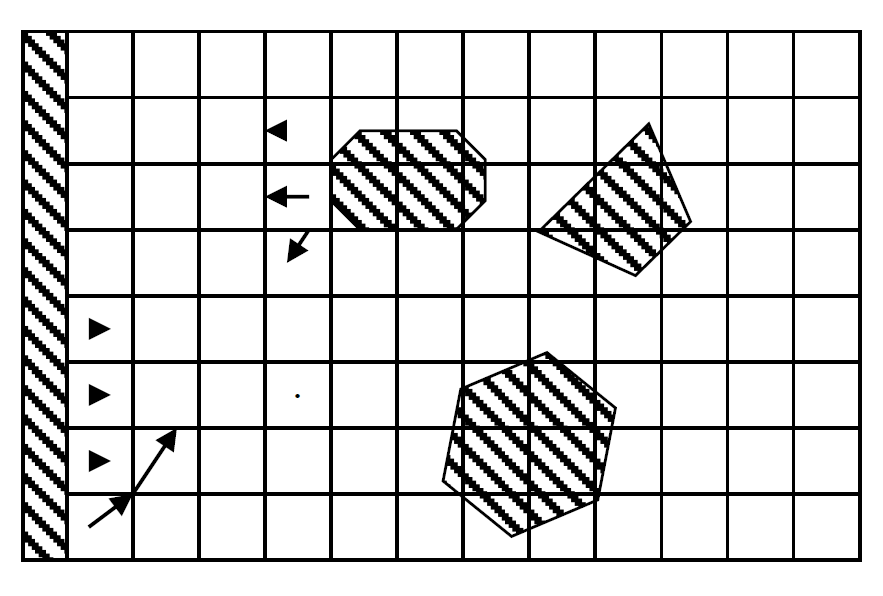
\includegraphics[width=0.5\textwidth]{images/img60.png}
	\label{figura60}
\end{figure}

Etc.

¿Cómo encontrar la fuerza de repulsión en cada celda?

\begin{figure}[h!]
	\centering
	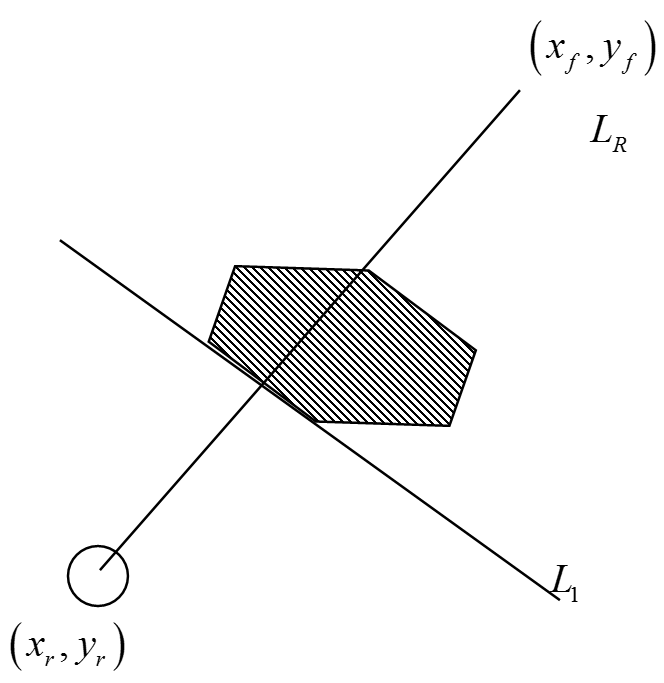
\includegraphics[width=0.5\textwidth]{images/img61.png}
	\label{figura61}
\end{figure}

El punto $x_r,y_r$ es el centro de la celda en donde se está (se asume que el robot está en el centro de la celda).

El punto $(x_f,y_f)$ es  un punto arbitrario (se quiere calcular para la mayor cantidad de direcciones posibles.
No es en línea sino que se hace offline).


\begin{flalign*}
\begin{aligned}
 L_1:\colon y=m_1x+b_1 \\
 L_R:y=m_Rx+b_R
\end{aligned}
\end{flalign*}


Nótese que 

\begin{flalign*}
\begin{aligned}
x_f=d\cos\phi+x_r \\
y_f=d\sin\phi+y_r
\end{aligned}
\end{flalign*}

Donde el ángulo es entre el eje x y la línea $L_R$.

Obs: se puede encontrar

$$
m=\dfrac{y_1-y_0}{x_1-x_0} \hspace{0.5cm} b=\frac{x_1y_0-y_1x_0}{x_1-x_0}
$$

Los puntos de intersección son

$$
x_{int}=\frac{b_r-b_1}{m_1-m_r} \hspace{0.5cm} y_{int}=m_r x_{int} + b_r
$$

Obsérvese que se tiene que cumplir que $x_{int} \in(x_0,x_1)$ y$y_{int} \in(y_0.y_1)$

\section{Cómo calcular el campo potencial para el caso de objetos desconocidos}

Lo anterior se hace offline y se alimenta al robot. Si hay objetos desconocidos:

\begin{figure}[h!]
	\centering
	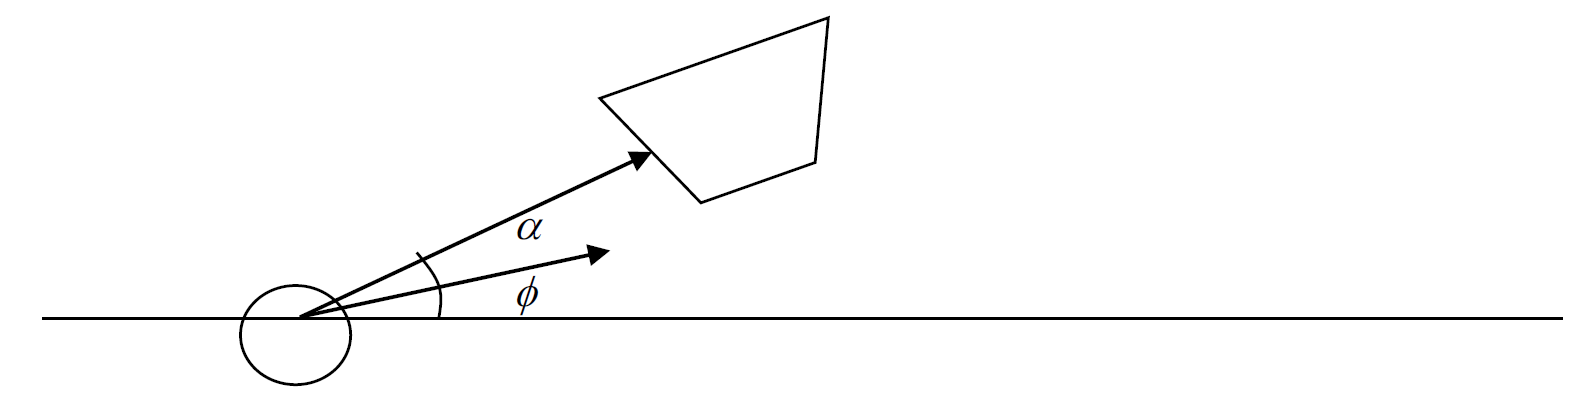
\includegraphics[width=0.5\textwidth]{images/img62.png}
	\label{figura62}
\end{figure}

\begin{scaja}
Tarea 1 \\
Usar Roc2. Poner obstáculos pickable en el medio. Programar un robot para encontrar esos obstáculos y que
los lleve a un lugar. Usar nada más la parte rectangular del mundo. El robot se mueve aleatoriamente. Tener
una pila que se vaya bajando.
\end{scaja}



¿Qué se quiere? \\
De $(x_{i-1},y_{i-1},\phi_{i-|})$ (donde está el robot) necesito llegar a $(x_i,y_i,\phi_i)$.

Obsérvese que: \\
 $x_i=x_{i-1}+x_i \cos(\phi_i)
 y_i=y_{i-1}+x_i \sin(\phi_i)
 $
 
donde:

$
\phi=\phi_{i-1}+\phi_i \\
\phi=\arctan\ (\frac{y_i -y_{i-1}}{x_i -x_{i-1}})
$


Esto se conoce como \textbf{computación directa}.

Otra opción es:

$
x'_i= \dfrac{(x_i - x_{i-1}) + (y_i - y_{i-1})}{\cos(\phi_i) + \sin(\phi_i)}
$

$
\phi_i = \phi_i - \phi_{i-1}
$
y obviamente también se tiene que $x_i = \sqrt{(x_i - x_{i-1})^2 + (y_i - y_{i-1})^2 }$



Esto se llama \textbf{computación inversa} y es la que nos interesa.



\textbf{Ejemplo}



\begin{figure}[h!]
	\centering
	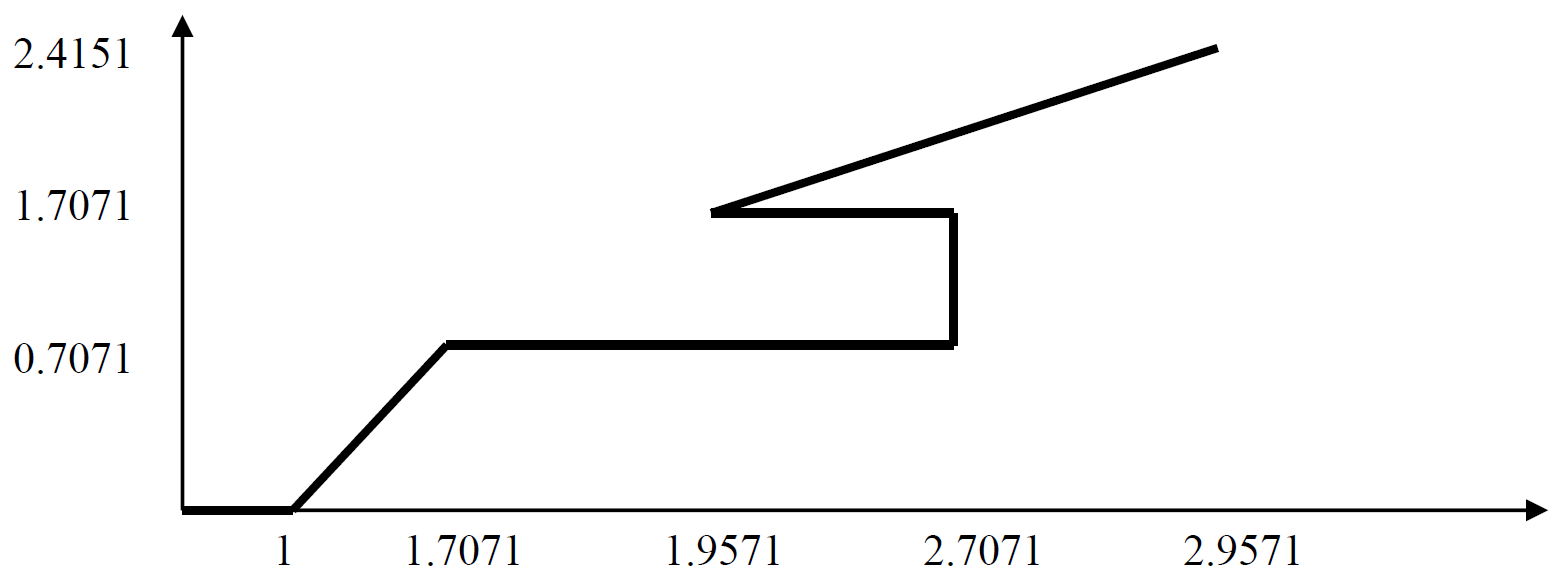
\includegraphics[width=0.5\textwidth]{images/img63.png}
	\label{figura63}
\end{figure}


\underline{Sup:} Los puntos los encontré con campos potenciales (recordar que el campo potencial da el vector de
movimiento:

$q_1=(x_i,y_i) = q_{i-1} - \delta f (q_{i-1})$
\\ \\
$ i=1 $ \\
$ x_0 = 0, \hspace{0.5cm} y_0=0, \hspace{0.5cm} \phi_0=0 $ \\
$x_i =1 \hspace{0.5cm} y_i=0 $

Por lo tanto: $\phi_1 =  arctan \, \left( \dfrac{y_1-y_0}{x_1-x_0} \right) = 0 \hspace{0.3cm} y \hspace{0.3cm} x_1 = \sqrt{(x_1-x_0)^2 + (y_1-y_0)^2} = 1.$ Y finalmente: \hspace{0.3cm} $\phi_i=\phi_i-\phi_{i-1} = 0$

Ad nauseam. \\
Los valores son:

\begin{figure}[h!]
	\centering
	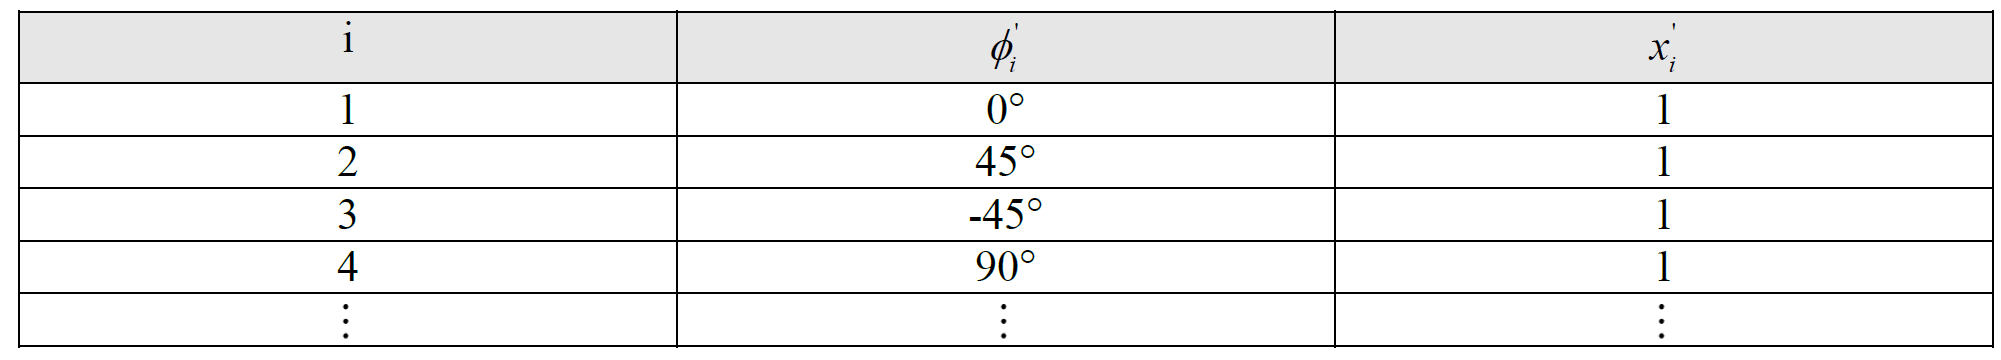
\includegraphics[width=0.5\textwidth]{images/img64.png}
	\label{figura64}
\end{figure}



\subsection{Trayectorias}

El robot casi siempre avanza en línea recta. \\
¿A qué velocidad debe ir el robot?

El robot está en $(x_{i-1},y_{i-1},\phi_{i-1}) $y quiero llegar a $(x_i,y_i)$ .¿Cómo voy a recorrer la distancia $x_i$?
Tengo $t_0$ y el tiempo $t_f$ (final).


\begin{figure}[h!]
	\centering
	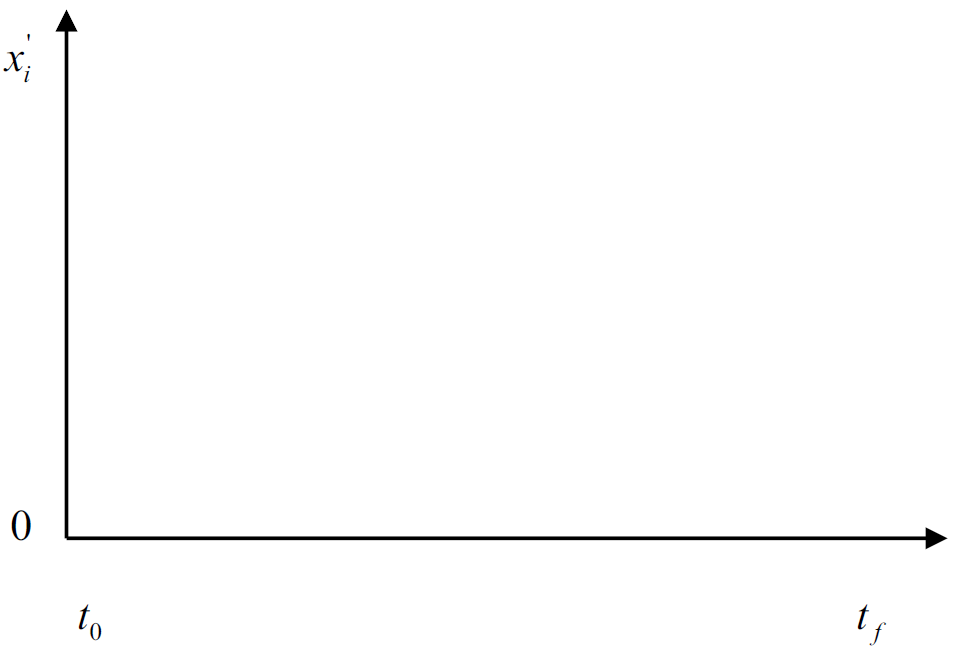
\includegraphics[width=0.5\textwidth]{images/img65.png}
	\label{figura65}
\end{figure}


Se quiere una función $f(t)$ que sea suave. Se asume que el robot está parado en ambos extremos.

$f(0)=0, \, f(t_f)= x_i' \hspace{0.3cm}$ [posiciones inicial y final]

$f'(0)=0, \, f'(t_f)= x_i $ \hspace{0.3cm}[velocidades inicial y final]


Asumiendo una relación cúbica:

$f(t)=a_0 +a_it + a_2 t^2 + a_3 t^3 \, f'(t_f)= x_i$

$f'(t)=a_1 + 2a_2t + 3a_3 t^2$

$f''(t)=2a_2 + 6a_3t$

Se encuentran:

$a_0, a_1=0, a_2=\dfrac{3x_i}{t_f^2},a_2=\dfrac{-2x_i}{t_f^3}$. La ecuación es entonces:
$$
f(t)=\dfrac{3x_i}{t_{f}^2}t^2 - \dfrac{2x'_{i}}{t_{f}^2} t^3
$$

$$
f'(t)=\dfrac{6x_i}{t_{f}^2}t -  \dfrac{6x'_{i}}{t_{f}^2} t^2
$$

$$
f''(t)=\dfrac{6x_i}{t_{f}^2}- \dfrac{12x'_{i}}{t_{f}^2} t
$$

\begin{ejemplo}
	
	
	Suponer $ t_f = 3 \,  x_1=1$ \\
	Entonces
	
	$$f(t)=\dfrac{1}{3}t^2 - \dfrac{2}{27}t^3
	$$
	
	$$f'(t)=\dfrac{2}{3}t - \dfrac{6}{27}t^2$$
	
	$$f''(t)=\dfrac{2}{3} - \dfrac{12}{27}t$$
	
\end{ejemplo}


\begin{figure}[h!]
	\centering
	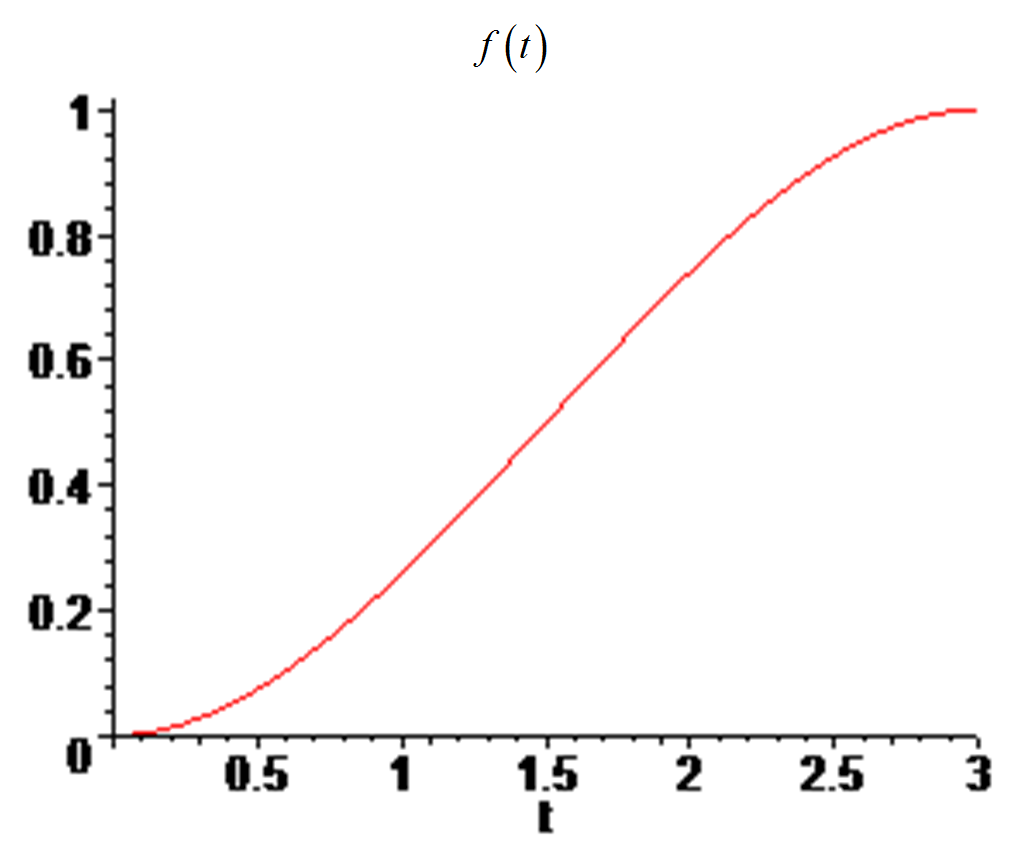
\includegraphics[width=0.5\textwidth]{images/img66.png}
	\label{figura66}
\end{figure}


$$
f'(t)$$
\begin{figure}[h!]
	\centering
	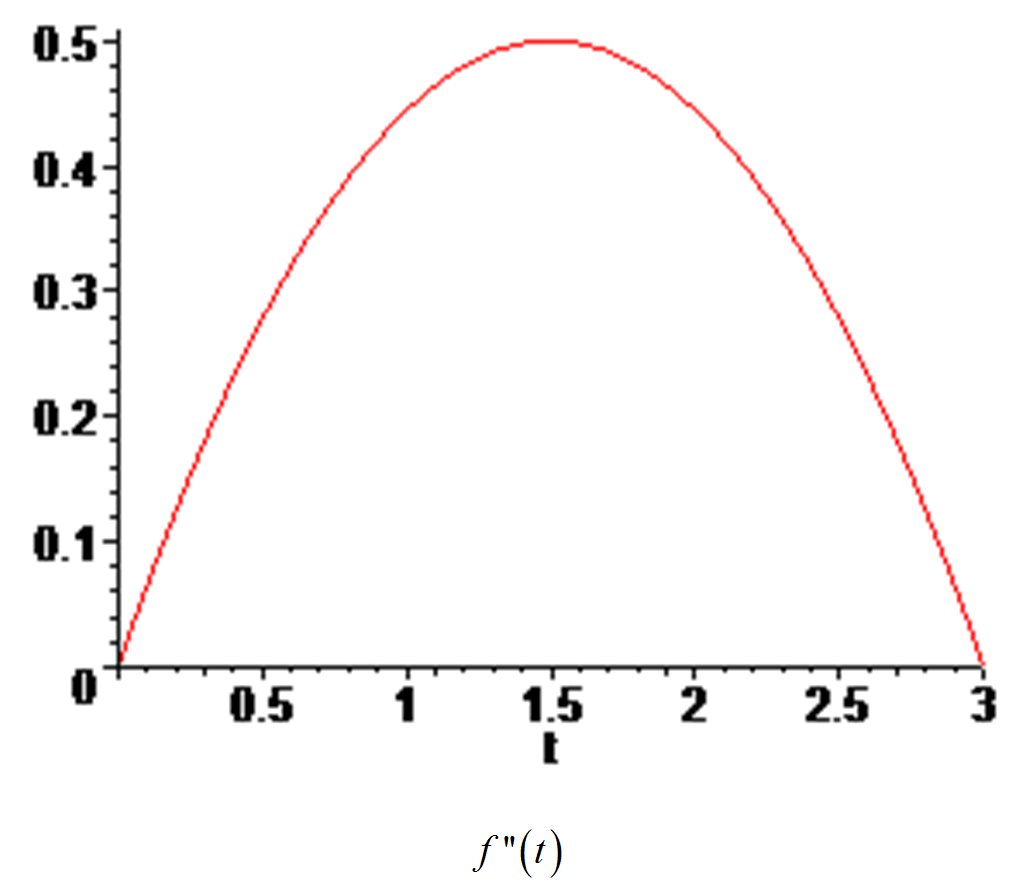
\includegraphics[width=0.5\textwidth]{images/img67.png}
	\label{figura67}
\end{figure}


\begin{figure}[h!]
	\centering
	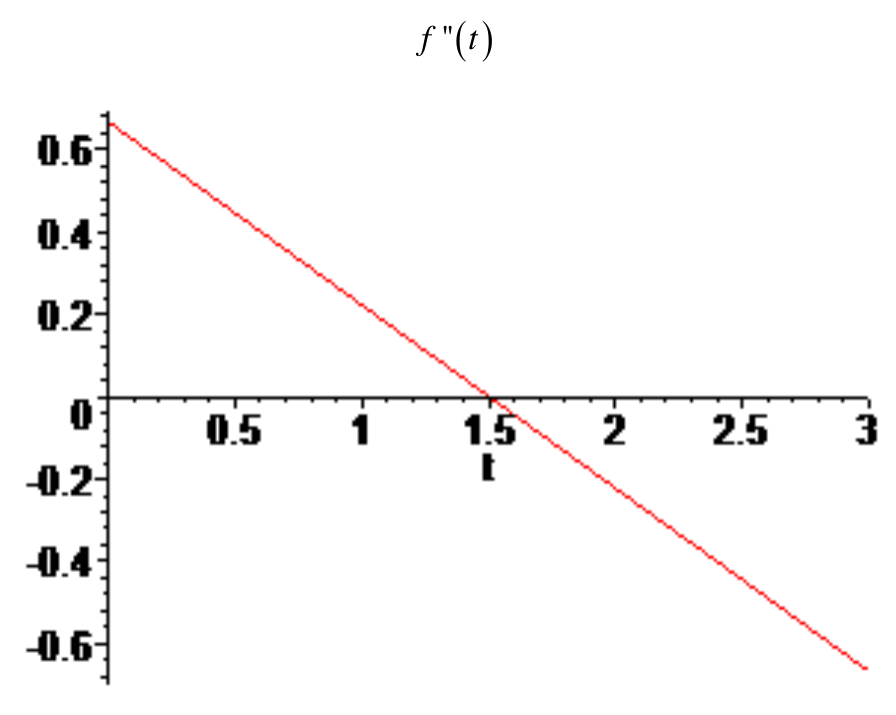
\includegraphics[width=0.5\textwidth]{images/img68.png}
	\label{figura68}
\end{figure}


En Roc2 para mover es:

mv $x'_i \hspace{0.3cm} \phi_i\hspace{0.3cm}t_f$

donde la primera está dada en decímetros y el ángulo en radianes y el tiempo en segundos.

En Roc2 las funciones cinemáticas se encuentran en el archivo Roc2UserMv.

\underline{\textit{Cómo relajar el supuesto de la velocidad final 0}}

Suavizar la trayectoria.

\begin{scaja} 
	
	Una forma: Le ajustas una parábola a la esquinita
	$y=y_0 + (x-x_0)^2$ con $x_b \leq x \leq x_f $ puntos pre-escogidos.
	
	\vspace{5mm}
	
	Otra forma: linearizar (segmentitos de recta).
	
\end{scaja}

\textbf{Rotar y trasladar}

polygon type-object $(x0,  y0, x1, \, y1, \, x2, \, y2, \, ... yn yn)$
position \textit{room} type-object name $xc yc theta ) \leftarrow$ esta función traslada a xc, yc y rota theta
Type-object define un objeto genérico, podemos definir varios objetos (de ese tipo).

\vspace{5mm}
Dados $(x_p,y_p)$


$ x= x_p \cos\alpha - y_p \sin\alpha +x_c $

$y = y_p \cos\alpha + x_p \sin\alpha +y_c$

Donde $x_c$, $y_c$ es el punto fijo sobre el que se está girando.

\begin{ejemplo}
	Polygon mesa $1 \, 0 \, 0\, 0\, 2\, 2\, 2\, 2\, 0$ \\	
	Position salon mesa1 mesa\_principal 44 $\frac{\pi}{4}$
\end{ejemplo}

Entonces:

\begin{figure}[h!]
	\centering
	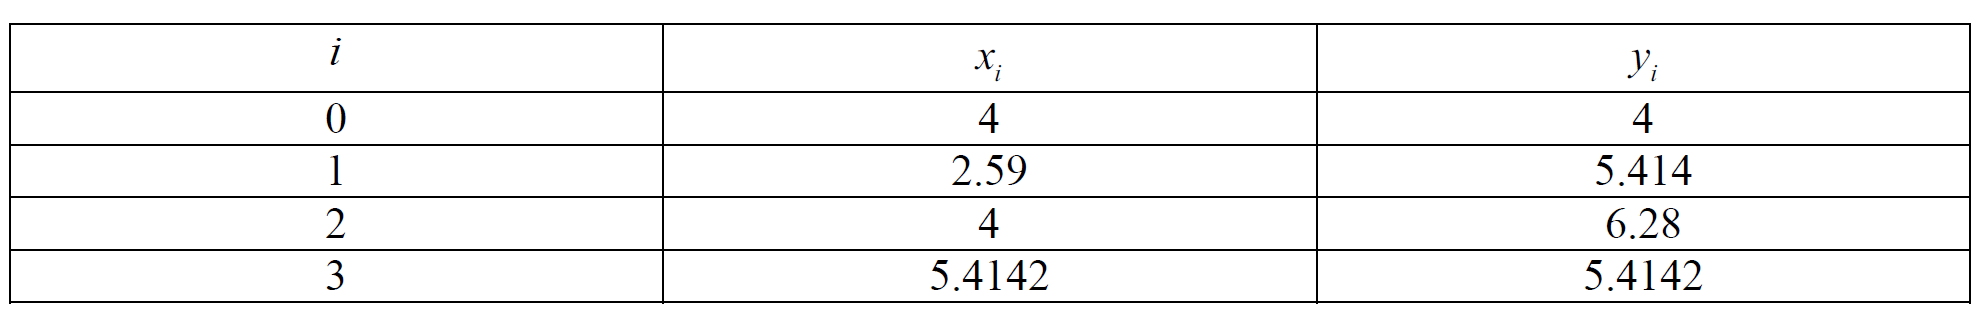
\includegraphics[width=0.5\textwidth]{images/img69.png}
	\label{figura69}
\end{figure}

\textbf{Ancho del robot}
Se necesita considerar el ancho del robot. Por lo menos, ensanchar los obstáculos conocidos en el radio del
robot.
¿Cómo hacer con los desconocidos? De la lectura del sonar, restarle el radio del robot.

\section{Escalamiento de polígonos}

Suponer (0, 2), (1,3), (2, 2), (1,1) un polígono.


\begin{enumerate}[1.]
	\item Encontrar el centroide
	\item Moverlo al origen
	\item Multiplicar
	\item Volverlo a mover al centroide.
\end{enumerate}


Con $\lambda =2$


$P_esc = \lambda (P - C) + C$

$P = \{(-1,2),(1,4),(3,2),(1,0)\}$

\begin{scaja}
	\textbf{Siguiente tarea}
	
	El mundo tiene mesas y otros dos objetos tipo, puestas y rotadas.
	
	Objetos fijos: sillones, mesas, cajas, etc. (al menos 3)
	\\
	
	Descomponer el mundo en celdas.
	\\
	
	Calcular los vectores de repulsión en cada celda.
	Si el centroide de la celda queda dentro del obstáculo, está ocupada
	Hacer una “estrella” hacia todas las direcciones y calcular si la intersección con algo es menor o igual a d0.
	\\
	La repulsión total es la suma.
	\\	
	
	Tres archivos: 1) objetos tipo 2) posiciones objetos réplica 3) archivo final .WRL con la descripción del
	mundo.
\end{scaja}


\textbf{Verificación de si un punto está dentro o fuera de un polígono}

\begin{figure}[h!]
	\centering
	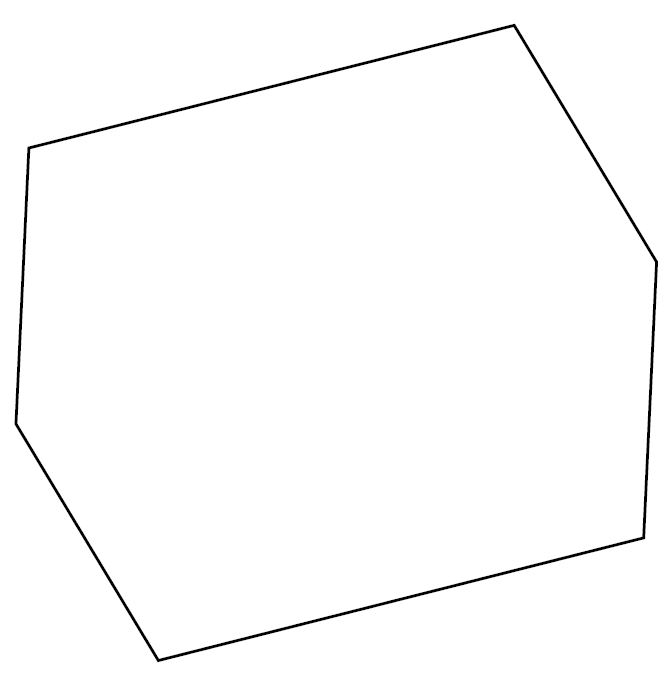
\includegraphics[width=0.5\textwidth]{images/img70.png}
	\label{figura70}
\end{figure}
	\break

Ecuación paramétrica de la recta
$
x = x_0 + (x_1 - x_0)t \\
y = y_0 + (y_1 - y_0)t \\
t \in (0,1)
$
Los puntos de la ecuación general

$
(y_0 - y_1)x + (x_1 - x_0)y + (x_oy_1 - x_1y_0) = 0
$

Puntos que cumplen esta ecuación, están en la línea.
\\ Puntos que evalúan >0, caen a la izquierda. \\ Puntos que evalúan <0, caen a la derecha.

\textbf{Problema de los campos potenciales}
\\ Por ejemplo un mínimo local

\begin{figure}[h!]
	\centering
	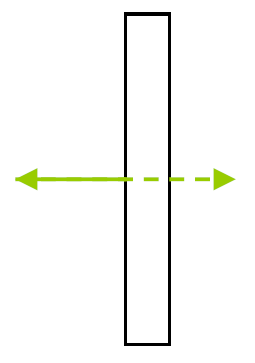
\includegraphics[width=0.5\textwidth]{images/img71.png}
	\label{figura71}
\end{figure}
\break


El vector resultante es 0 y el robot se queda inmóvil o en un ciclo.

\section{Comportamientos con Redes Neuronales}

Redes neuronales: 1943 $\rightarrow$  McCullock


Una red neuronal es un modelo matemático de cómo funciona una neurona.

Una neurona está conectada a otras neuronas.

\begin{figure}[h!]
	\centering
	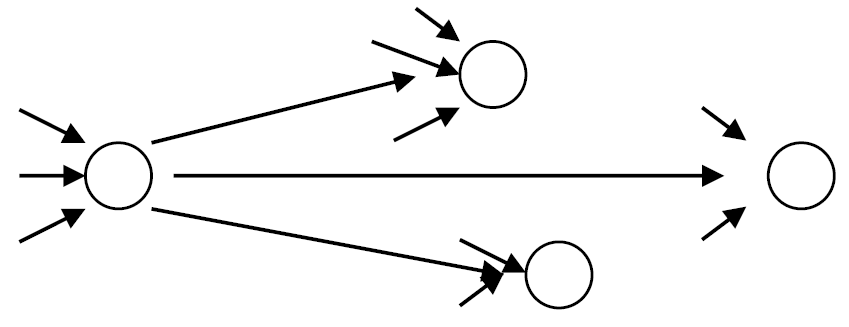
\includegraphics[width=0.5\textwidth]{images/img72.png}
	\label{figura72}
\end{figure}

La entrada a la red neuronal es una imagen (por ejemplo, la cámara del robot). Se puede entregar la
información en bruto o procesada.

Las conexiones se van uniendo por medio de aprendizaje.

Se entrena a la red para que siga los comportamientos, por ejemplo un coche autónomo. Para entrenarlo, se
puede poner a un conductor y hacer que la red aprenda los comportamientos de acuerdo a las imágenes.
La respuesta de la red es: para una cierta imagen, se giró a la izquierda violentamente; para otra imagen, se
giró ligeramente; etcétera.

También se puede hacer con información de sonares, etc.

Puedo hacer máquinas de estado con redes neuronales.

\begin{figure}[h!]
	\centering
	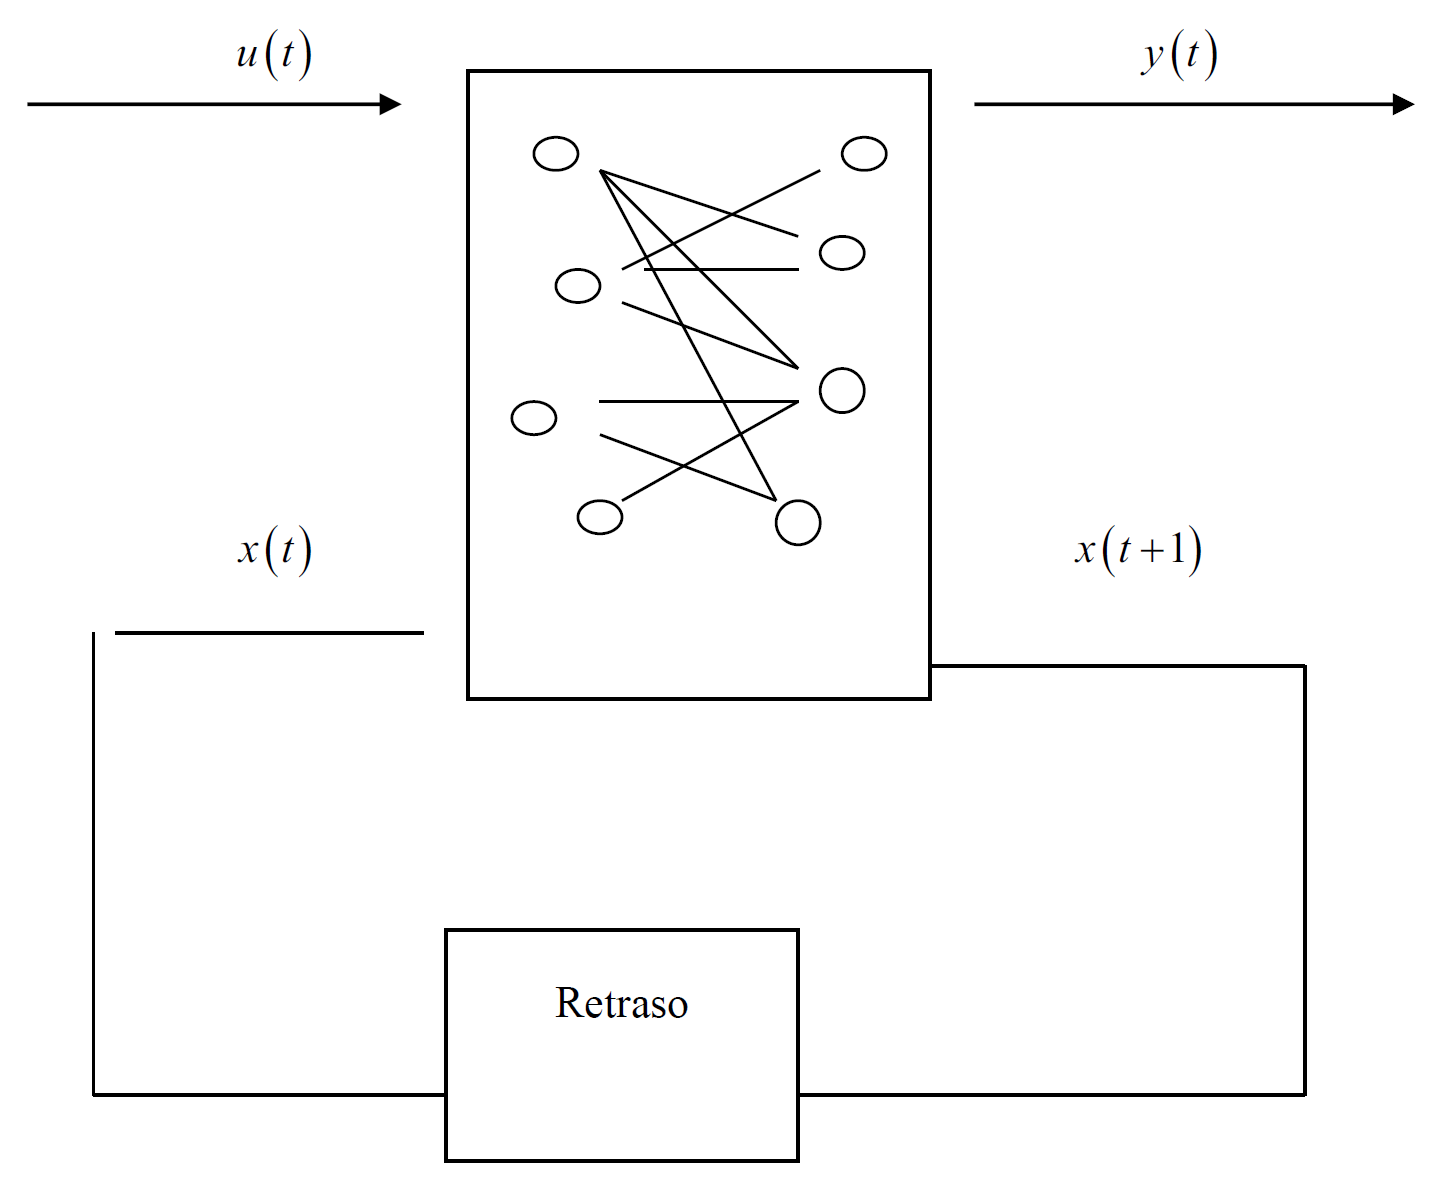
\includegraphics[width=0.5\textwidth]{images/img73.png}
	\label{figura73}
\end{figure}

\textbf{Modelo}

Por cada neurona se tiene

$u = \sum_{i=1}^{n} w_i y_i + \theta $

Entradas: $ y_j \rightarrow $  vienen de otras neuronas
Pesos: $w_j$
Umbral de activación: $ \theta $

La salida de la neurona es la \textit{función de activación}

$$
a=f(u)
$$

Generalmente $ f(u) = \dfrac{1}{1 + e^(\dfrac{-u}{T})}$ (un sigmoide)

$T$ es una constante de temperatura. 


Resulta que f es la solución de la ecuación diferencial 

$$
\dfrac{dy}{du} = \dfrac{y(1-y)}{T}
$$


\section{Topología de Redes Neuronales}

¿Qué pasa con la topología de redes neuronales (muchas neuronas)?

\begin{figure}[h!]
	\centering
	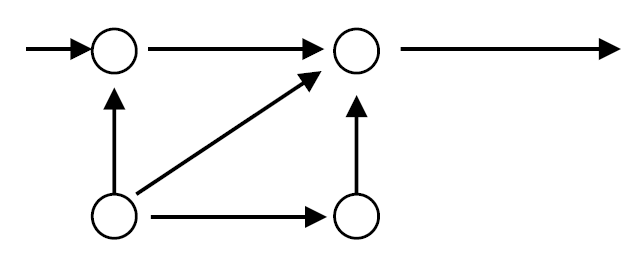
\includegraphics[width=0.5\textwidth]{images/img74.png}
	\label{figura74}
\end{figure}
\break

Topología acíclica (no hay retroalimentación de la salida hacia otra interna) $\rightarrow$ el dígrafo es acíclico.

\begin{figure}[h!]
	\centering
	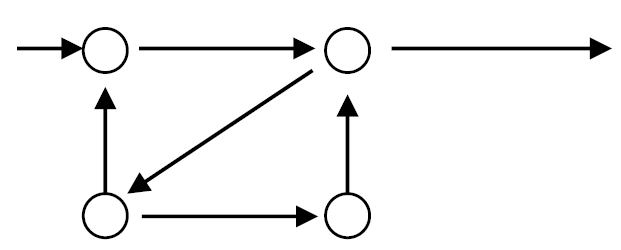
\includegraphics[width=0.5\textwidth]{images/img75.png}
	\label{figura75}
\end{figure}


Topología cíclica (con retroalimentación) $\rightarrow$ el dígrafo es cíclico
Estos fueron los primeros modelos de redes neuronales.

\section{Modelo del Perceptrón}

$
u(x) = \sum_{i=1}^{n} w_i x_i + w_0 
$
y

$
y(x) = \begin{cases}
1, \hspace{0.3cm} u(x) \geq 0    \\
0,\hspace{0.3cm}   u(x) < 0  
\end{cases}
$

Este modelo es utilizado para \textit{detección y clasificación}.

Si las características de la entrada $x$ es cercano a $w$ tal que su producto interno $x^Tw$ es mayor que un
umbral $-w_0$, entonces la salida es 1, indicando la detección de un objetivo.


\begin{ejemplo}
	Dos neuronas, una que representa una mesa y otra una silla.
	Las dos tienen las mismas entradas, que son características invariantes a distancia y orientación. La salida
	debe de ser 1 para la de la silla y 0 para la de la mesa.
\end{ejemplo}

\begin{nota} Entrenar a una red neuronal es encontrar los pesos. \end{nota}


Minsky y Shannon

Shannon propone la matemática booleana y notación binaria en las computadoras.
Wiener inventó el término \textit{cibernética} (el estudio de los sistemas – eléctricos, mecánicos, sociales, etc. – y su control).


LEER ASIMOV Y PHILIP DICK

\section{Perceptrón multicapas}

Capa de entradas
Capa intermedia
Capa de salida

\begin{figure}[h!]
	\centering
	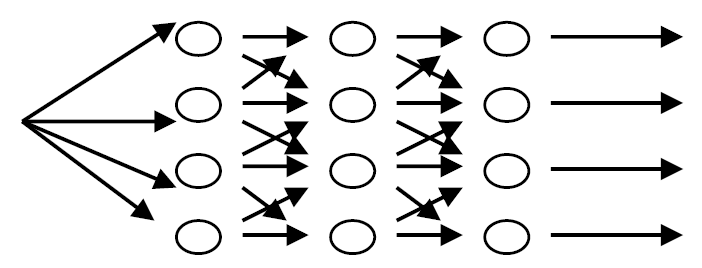
\includegraphics[width=0.5\textwidth]{images/img76.png}
	\label{figura76}
\end{figure}

La capa de entrada tiene M neuronas.
La capa intermedia se conoce como \textit{capa oculta} y tiene H neuronas.
La capa de salida tiene N neuronas.

El objetivo es encontrar los pesos que minimicen el error cuadrático medio.


Cada salida de las neuronas de salidas es un objetivo de clasificación.

\begin{ejemplo}
	
¿Cómo encontrar los pesos?

Tres entradas, una neurona de entrada.

$u=Wx$ donde $x = [1 \hspace{0.3cm} x_1 \hspace{0.3cm}  x_2]^T \hspace{0.3cm} y \hspace{0.3cm} W= [W_0 \hspace{0.3cm} w_1 \hspace{0.3cm} W_2]$
\\

Encontrar unos pesos que dado un objetivo $d_k$ e vaya actualizando con la característica que $\varepsilon \rightarrow 0$. Se
tendrán K muestras de entrenamiento $(x_k,d_k)$; salidas $z_k$ y un error total $E= \sum_{i=1}^{K}  \varepsilon_k^2$, donde $\varepsilon= d_k - z_k$.
\\

$d_k \in (0.1)$ generalmente. 

\end{ejemplo}


\begin{figure}[h!]
	\centering
	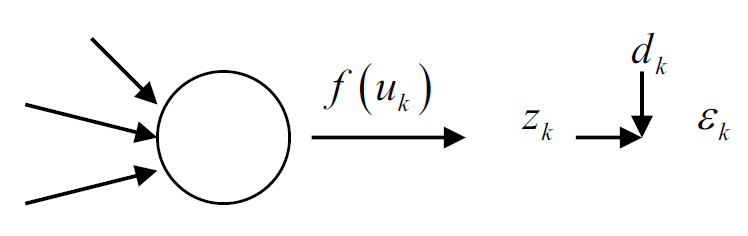
\includegraphics[width=0.5\textwidth]{images/img77.png}
	\label{figura77}
\end{figure}

Obsérvese que $z_k = f(Wx_k)$.

El objetivo final es minimizar la función $E$ respecto a $W$. 

La solución es no lineal si f es una función sigmoide, por lo que generalmente se realiza la minimización con
iteraciones:

$ W_{t+1} = W_t + \Delta W_t
$

Por método de \textit{steepest descent:}
$\Delta W_t= -\eta \dfrac{dE}{dW}
$

Solución
\\

$$
\dfrac{dE}{dW_i} = -2  \sum_{k=1}^{K}
(d_k - z_k) (\dfrac{-dZ_k}{dw_i})
$$

Obsérvese que

$$\dfrac{-dz_k}{dw_i} = \dfrac{df(u)}{dW_i} = \dfrac{df(u)}{du} \dfrac{du}{dw_i} = f'(u) \dfrac{du}{dw_i} = f'(u) x_i
$$

Por lo que

$$
\dfrac{dE}{dW_i} = 2 \sum_{k=1}^{K} (d_k - z_k) f'(u) x_i
$$

Se denota $\delta_k = [d_k - x_k] f'(u_k)$ y entonces

\begin{scaja}
	$$ w_i(t + 1) = w_i(t) + \eta \sum_{i=1}^{K} \delta_k x_i (k) $$
\end{scaja}

En particular si $f(u)$ es el sigmoide, entonces

$\delta_k=[d_k - z_k] \, z_k \,  (1-z_k)\, \alpha := \dfrac{\partial E}{\partial u}
$

\begin{scaja}
	$$ \dfrac{\partial E}{\partial u} = -2 \sum_{i=1}^{K} [d_k - z_k] \dfrac{dZ_k}{du} $$ y ademas $$\dfrac{dz_k}{du}= \dfrac{f(u)[1 - f(u)]}{T}
	$$.   \\  Por lo tanto, 
	$$
	\dfrac{\partial E}{\partial u} = -2 \sum_{i=1}^{K} [d_k - z_k] f(u) [1 - f(u)] = \dfrac{-2}{T} -2 \sum_{i=1}^{K} [d_k - z_k] \, z_k \, [1-z_k]. 
	$$
\begin{center}
	QED
\end{center}	
\end{scaja}

El proceso se debe hacer hasta que $E\textless \epsilon$


\section{Cómo extender para un perceptrón multicapas}

Se tienen:

K muestras de entrenamiento
L capas

$W_{ij}^L$ es el peso de la neurona $i$ a la neurona $j$ en la capa L y en la iteración $t$.

\textit{Propagación de error:}

\begin{figure}[h!]
	\centering
	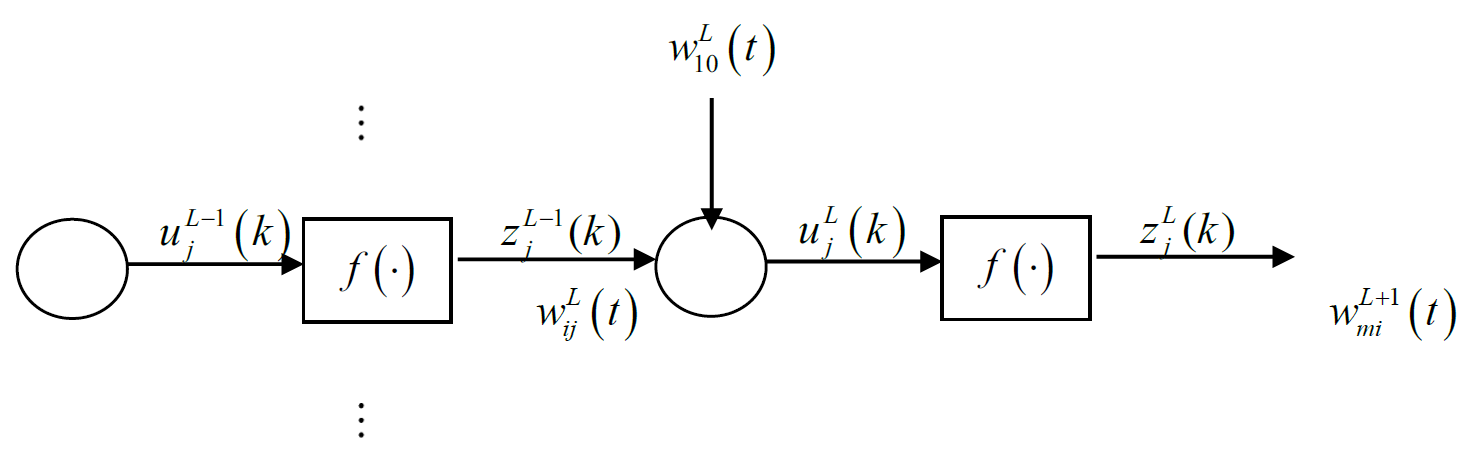
\includegraphics[width=0.5\textwidth]{images/img78.png}
	\label{figura78}
\end{figure}

El objetivo es (de nuevo) encontrar $w_ij$ de cada capa que minimicen el error cuadrático medio.

%$$ \dfrac{dE}{dw_ij^L} = -2 \sum_{i=1}^{K} \dfrac{dE}{du_i^L (k)} \dfrac{du_i^L(k)}{dw_ij^} = -2 \sum_{k=1}^{K} \delta_i^L (k) \dfrac{du_i^L(k)}{dw_ij^L}$$

Pero dado que

$
\dfrac{du_i^L (k)}{dw_{ij}^L} = \dfrac{d}{dw_{ij}^L}  \sum_{m=1}^{M} \hspace{0.2cm} w_{im}^L \hspace{0.2cm} z_{m}^{L-1} (k) 
$

%avances hasta hoy 17 